
We have created a publicly available dataset and project website which users, developers and researchers may use. In the following sections, we describe the dataset and website.



\subsection{Dataset}


Our data set is available from our publicly accessible GitHub repo\footnote{\ifisnopii https://github.com/DroidDarwin \else https://github.com/-Hidden- \fi} (linked from the \ifisnopii Darwin \else -Hidden- \fi website), which includes the scripts used for collecting apps and invoking the static analysis tools. The SQLite database with our complete results is updated on a regular basis from our scanning and analysis application. The goal of this dataset is to allow future researchers to both learn from and expand upon our work. This data includes the following fields for each app:

\begin{itemize}
    \setlength{\itemsep}{0pt} %Cut down on spacing for the different items in the list
    \setlength{\parskip}{0pt} %Cut down on spacing for the different items in the list
    \setlength{\parsep}{0pt}  %Cut down on spacing for the different items in the list

  \item Name
  \item Version
  \item Genre
  \item Number of downloads from Google Play
  \item Publication date on Google Play
  \item Google Play user rating
  \item Overprivileges
  \item Underprivileges
  \item Count of Jlint reported defects
  \item Count of CheckStyle coding standards mistakes
  \item Application size
  \item Application Permissions
  \item Count of .java files
  \item Vulnerability risk score from AndroRisk
  \item Code clone count from Simcad
\end{itemize}

\todo{really add to this section. What more could we add?}


% How much data do we have. Show a small table with commits?
We performed static analysis on \hl{68,514} apps collected from Google Play. Overall, these apps contained \hl{428,514} permissions, \hl{101,113} overprivileges and \hl{166,948} underprivileges.


Possible uses of data are innumerable, with some including further work on comparing security (AndroRisk and overpriviledges)

%   - Data to show in a table or something pretty
% How many apps do we have several versions of?


\subsection{Website}

%%% Tell the story of how the website can be used

Our project website (\textbf{\ifisnopii http://darwin.rit.edu \else http://xxx.hidden.edu \fi}) contains information about our project, links to our GitHub repository, and a robust reporting tool which will allow users to create their own data sets from over 68,000 analyzed applications. As show in Figure~\ref{fig:website1}, user's may search for individual apps to view specific information about the app as taken from Google Play, and from our static analysis results.

 \begin{figure}[ht!]
\centering
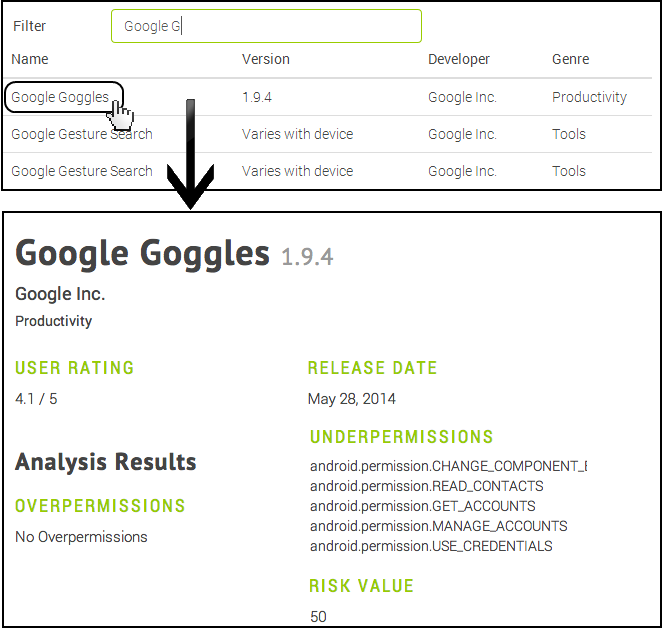
\includegraphics[width=\columnwidth, angle = 0]{images/screenshot3.png}
\caption{\ifisnopii darwin.rit.edu \else xxx.hidden.edu \fi Website Reporting Tool}
\label{fig:website1}
\end{figure}


The website also includes several data driven result sets about apps at a more aggregate level. Figure~\ref{fig:overprivappsByGenre} shows the percentage of apps in the top 5 genres that contain at least 1 overprivilege.

 \begin{figure}[ht!]
\centering
%\frame{ % Create frame around image
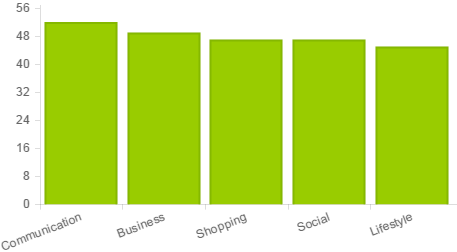
\includegraphics[scale=.7]{images/overprivsByGenre.png}
%} % end frame around image
\caption{Overprivileged Apps By Genre from Project Website\todo{frame?}\todo{update with new data}}
\label{fig:overprivappsByGenre}
\end{figure}


% http://darwin.rit.edu/reports
16 prebuilt reports in .csv format are available in several areas including the rate at which two overprivileges appear together in all applications, the percentage of times each overprivilege occurs in all applications, and the percentage of times each overprivilege occurs in all applications.






\todo{really add to this section}
\dan{how long should this section be?}

